Αρχικά, θα εξετάσουμε την περίπτωση του «καθαρού» MPI, ξεκινώντας από τον κώδικα.
\section{Επεξήγηση κώδικα}

\subsection{Macros} \label{sec:macros}

\begin{tcolorbox}
\begin{minted}{C}
#define SIZE 8
#define NDIMS 2
#define DEBUG_COORDINATES
#define DEBUG_GRID
\end{minted}
\end{tcolorbox}

\begin{multicols}{2}
Προκειμένου να τρέξει σωστά το πρόγραμμά μας, χρειαζόμαστε τα παραπάνω macros. 
Το macro \textbf{SIZE} αναφέρεται στο μέγεθος του πίνακα ο οποίος θα φιλοξενήσει το Game of Life. Στο μέγεθος αυτό δεν περιλαμβάνονται οι άλω σειρές και στήλες, οπότε και θα προστεθούν στην πορεία.Το macro \textbf{NDIMS} αναφέρεται στο πλήθος των διαστάσεων που θέλουμε να έχει η καρτεσιανή τοπολογία. Στην περίπτωσή μας, χρειαζόμαστε δύο διαστάσεις, οπότε και η τιμή του macro θα παραμείνει ίδια καθόλη τη διάρκεια των δοκιμών.Τα macros \textbf{DEBUG\_COORDINATES} και \textbf{DEBUG\_GRID} χρησιμοποιούνται μόνο για debugging της εφαρμογής, αφού χρησιμοποιούνται για να τυπώνεται σε κάθε επανάληψη το πλέγμα του παιχνιδιού. Θα χρησιμοποιηθούν μόνο για επαλήθευση της ορθότητας των αποτελεσμάτων με μικρά μεγέθη πίνακα, και στην συνέχεια θα απενεργοποιηθούν για τις τελικές μετρήσεις.
\end{multicols}

\subsection{Συναρτήσεις}

\begin{tcolorbox}
\begin{minted}{C}
void Initial_state(int rows, int columns, char *first_generation, char *first_generation_copy, int seed);
void Print_grid(int rows, int columns, char *life);
void inline Next_generation_inner(int rows, int columns, char *life, char *life_copy);
void inline Next_generation_outer(int rows, int columns, char *life, char *life_copy);
void inline Swap(char **a, char **b);
\end{minted}
\end{tcolorbox}

\begin{multicols}{2}
Η συνάρτηση \textbf{Initial\_state} καλείται μία φορά, έξω από το κύριο loop. Σκοπός της είναι η αρχικοποίηση του πλέγματος της κάθε MPI διεργασίας με τυχαίους ζωντανούς και νεκρούς οργανισμούς, οι οποίοι παράγονται με την βοήθεια της μεταβλητής \mintinline{C}{int seed}. Οι άλω σειρές και στήλες αρχικοποιούνται με την τιμή 0. Η συνάρτηση \textbf{Print\_grid} τυπώνει το πλέγμα της κάθε διεργασίας στο output αρχείο. Επειδή το I/O επιφέρει μεγάλες καθυστερήσεις στην εκτέλεση του προγράμματος, η συνάρτηση αυτή χρησιμοποιείται μόνο για debugging και επαλήθευση της ορθότητας των αποτελεσμάτων. Οι συναρτήσεις \textbf{Next\_generation\_inner} και \textbf{Next\_generation\_outer } υπολογίζουν σε κάθε επανάληψη την επόμενη γενιά. Η πρώτη υπολογίζει μόνο τα εσωτερικά στοιχεία του πλέγματος --- και ενώ περιμένουμε την παραλαβή των άλω στοιχείων --- ο υπολογισμός των οποίων δεν εξαρτάται από τις άλω σειρές και στήλες. Αντίστοιχα, η δεύτερη υπολογίζει τα εξωτερικά στοιχεία του πλέγματος μετά από την παραλαβή των άλω στοιχείων. Η συνάρτηση \textbf{Swap} καλείται στο τέλος κάθε επανάληψης και ανταλλάσει τους pointers των δύο πινάκων, ώστε να αποφεύγεται η αντιγραφή από τον ένα πίνακα στον άλλο σε κάθε επανάληψη. Οι τρεις τελευταίες συναρτήσεις που αναφέρθηκαν, έχουν δηλωθεί ως \mintinline{C}{inline}, επειδή χρησιμοποιούνται σε κάθε επανάληψη του κύριου loop, και θέλουμε να αποφευχθούν τα branch instructions τα οποία επιφέρουν και καθυστερήσεις στην εκτέλεση του προγράμματος.
\end{multicols}

\clearpage

\subsection{Η συνάρτηση main()}
\subsubsection{Αρχικοποίηση μεταβλητών}
Στη συνέχεια θα εξετάσουμε τη ροή της συνάρτησης main, όπου χρησιμοποιούνται και όλες οι προαναφερθείσες συναρτήσεις για την υλοποίηση του Game of Life. Αρχικά έχουμε τη δήλωση όλων των μεταβλητών που είναι απαραίτητες για την κατανομή των διεργασιών σε καρτεσιανή τοπολογία.

\begin{tcolorbox}
\begin{minted}[breakindentnchars=31]{C}
/*******************************************************************************
* ARRAYS FOR THE CARTESIAN TOPOLOGY
* dim_size - Array with two elements
*     dim_size[0]  - How many processes will be in each row
*     dim_size[1]  - How many processes will be in each column
*
* periods                    - Array with two elements, for the periodicity of the two dimensions
* coords                     - Array with two elements, holding the coordinates of the current process
* north, east etc.           - The coordinates of each of our eight neighbors
********************************************************************************/

int dim_size[NDIMS], periods[NDIMS], coords[NDIMS];
int north[NDIMS], east[NDIMS], south[NDIMS], west[NDIMS],
     northeast[NDIMS], southeast[NDIMS], southwest[NDIMS], northwest[NDIMS];

/********************************************************************************
* VARIABLES FOR THE CARTESIAN TOPOLOGY
* reorder                    - Indicates if MPI can rearrange the processes more efficiently among the processors
* rank                       - Process rank
* processes                  - The total number of processes in the communicator
* rows                       - The number of rows of the local 2D matrix
* columns                    - The number of columns of the local 2D matrix
* seed                       - The seed used to randomly create the first generation
* north_rank, east_rank etc. - The ranks of the neighbors
* cartesian2D                - Our new custom Communicator
*********************************************************************************/

int            reorder, rank, processes, rows, columns, seed;
int            north_rank, east_rank, south_rank, west_rank,
               northeast_rank, southeast_rank, southwest_rank, northwest_rank;
MPI_Comm       cartesian2D;
\end{minted}
\end{tcolorbox}

\begin{multicols}{2}
Αρχικά, έχουμε τους πίνακες dim\_size, periods, coords, north, east κλπ. Όλοι οι πίνακες έχουν μέγεθος NDIMS, δηλαδή $2$. Ο πίνακας \textbf{dim\_size } περιέχει ως πρώτο του στοιχείο τον αριθμό των MPI processes που θα αντιστοιχούν σε κάθε γραμμή του πλέγματος, και ως δεύτερο στοιχείο τον αριθμό των MPI processes σε κάθε στήλη του πλέγματος. Πχ, για $8$ συνολικά MPI processes, το πρώτο στοιχείο πιθανόν να έχει την τιμή $4$, και το δεύτερο την τιμή $2$. Άρα τα processes κατανέμονται ομοιόμορφα σε μία $2*4$ διάταξη. Εάν πάλι ο αριθμός των processes είναι τέλειο τετράγωνο, πχ. $9$, τότε η κατανομή γίνεται ομοιόμορφα σε μία $3*3$ διάταξη (Σχήμα \ref{fig:cartesian}). Όπως θα δούμε παρακάτω, οι διατάξεις αυτές δεν αποφασίζονται από εμάς, αλλά αφήνουμε το MPI να αναλάβει την κατανομή, με τον τρόπο που αυτό θα θεωρήσει βέλτιστο.
\end{multicols}

\begin{figure}[h]
\centering
\begin{minipage}{0.45\textwidth}
\centering
\begin{tabular}{cc}
    process0 & process1 \\
    process2 & process3 \\
    process4 & process5 \\
    process6 & process7
\end{tabular}
\subcaption{Διάταξη $2*4$}
\end{minipage}\hfill
\begin{minipage}{0.45\textwidth}
\centering
\begin{tabular}{ccc}
    process0 & process1 & process2 \\
    process3 & process4 & process5 \\
    process6 & process7 & process8
\end{tabular}
\subcaption{Διάταξη $3*3$}
\end{minipage}
\caption{Δύο διαφορετικές διατάξεις}
\label{fig:cartesian}
\end{figure}

\begin{multicols}{2}
Ο πίνακας \textbf{periods} χρησιμοποιείται από το MPI για να ελέγξει την περιοδικότητα των δύο διαστάσεων. Και οι δύο του θέσεις θα λάβουν την τιμή $1$, η οποία και δεν θα αλλάξει καθόλη τη διάρκεια της εκτέλεσης. Η τιμή $1$ και στις δύο θέσεις, δηλώνει πως έχουμε περιοδικότητα και στις δύο διαστάσεις, επομένως και το board του Game of Life θα είναι τόρος. Ο πίνακας \textbf{coords} περιέχει τις συντεταγμένες του εκάστοτε MPI process, με την τιμή στην πρώτη θέση να δίνει τη συντεταγμένη $x$, και την τιμή στη δεύτερη θέση να δίνει την συντεταγμένη $y$. Τέλος, οι πίνακες \textbf{north, east, south} κλπ, περιέχουν ο καθένας στις δύο του θέσεις τις συντεταγμές του αντίστοιχου γειτονικού MPI process, πχ ο πίνακας north περιέχεις τις συντεταγμένες της βόρειας διεργασίας. \par
Στη συνέχεια, έχουμε τις μεταβλητές που θα χρησιμοποιηθούν από το MPI για τη δημιουργία και λειτουργία της καρτεσιανής τοπολογίας. Η μεταβλητή \textbf{reorder} θα λάβει την τιμή $1$ και θα υποδείξει στο MPI πως είναι ελεύθερο να κατανείμει τις διεργασίες στους διαθέσιμους επεξεργαστές, όπως αυτό κρίνει βέλτιστο. Η μεταβλητή \textbf{rank} είναι ο βαθμός της τρέχουσας διεργασίας, και η μεταβλητή \textbf{processes} δηλώνει πόσες συνολικά διεργασίες θα χρησιμοποιήσει το πρόγραμμά μας. Οι μεταβλητές \textbf{rows και columns} δηλώνουν πόσες γραμμές και στήλες θα έχει το τοπικό πλέγμα της κάθε διεργασίας αντίστοιχα, και η μεταβλητή \textbf{seed} είναι ένας random seed που θα χρησιμοποιηθεί ως παράμετρος της συνάρτησης \mintinline{C}{Initial_state}, μόνο για την τυχαία παραγωγή της πρώτης γενιάς. \par
Οι μεταβλητές \textbf{north\_rank, east\_rank} κλπ, μας δείχνουν τους βαθμούς των γειτονικών διεργασιών. Τέλος, η μεταβλητή \textbf{cartesian2D} θα είναι ο καινούριος custom communicator που θα αποθηκεύσει τη νέα τοπολογία.
\end{multicols}

\clearpage

\begin{tcolorbox}
\begin{minted}[breakindentnchars=48]{C}
/***********************************************************************************
* VARIABLES FOR MPI
* row_datatype                                - Custom datatype to send/receive                                                             the halo rows
* column_datatype                             - Custom datatype to send/receive the halo columns
* receive_requests_even, receive_requests_odd - Arrays holding all the requests for receiving messages
* send_requests_even, send_requests_odd       - Arrays holding all the requests for sending messages
* statuses                                    - Array holding the output of the Waitall operation
* t1, t2                                      - Used by MPI_Wtime
* root                                        - Used to check if the number of processes is a perfect square
************************************************************************************/

MPI_Datatype   row_datatype, column_datatype;
MPI_Request    receive_requests_even[8], send_requests_even[8], 
                         receive_requests_odd[8], send_requests_odd[8];
MPI_Status     statuses[8];
double         t1, t2, root;
\end{minted}
\end{tcolorbox}

\begin{multicols}{2}
Στη συνέχεια εξετάζουμε τις μεταβλητές που θα χρησιμοποιηθούν από το MPI κατά τη διάρκεια του παιχνιδιού. Θα εφαρμοστεί persistent communication, αφού οι γειτονικές διεργασίες παραμένουν σταθερές καθόλη τη διάρκεια του παιχνιδιού. Επομένως, η καλύτερη μέθοδος είναι να ορίσουμε οσο το δυνατόν περισσότερες μεταβλητές μόνο μία φορά, και έξω από την κεντρική επανάληψη. \par
Αρχικά, οι μεταβλητές \textbf{row\_datatype και column\_datatype} ορίζουν custom MPI datatypes για την αποδοτική αποστολή και λήψη άλω γραμμών και στηλών αντίστοιχα. Οι πίνακες \textbf{receive\_requests\_even, send\_requests\_even, receive\_requests\_odd και send\_requests\_odd} έχουν όλοι μέγεθος $8$, και περιέχουν τα 8 custom receive και send requests της κάθε διεργασίας. Χρειαζόμαστε $8$ θέσεις σε κάθε πίνακα, επειδή τόσες είναι οι αποστολές και οι λήψεις διαφορετικών στοιχείων (βόρεια και νότια σειρά, ανατολική και δυτική στήλη, καθώς και $4$ γωνιακά στοιχεία). Επίσης, έχουμε δύο διαφορετικούς πίνακες για κάθε λειτουργία, με το επίθεμα odd και even. Τα requests που περιέχονται στον καθένα από αυτούς τους πίνακες, θα χρησιμοποιούνται ανάλογα με το αν το παιχνίδι βρίσκεται σε περιττή ή άρτια επανάληψη. Τον λόγο που αυτό είναι απαραίτητο, θα τον εξετάσουμε αργότερα. \par
Ο πίνακας \textbf{statuses} χρησιμοποιείται για να αποθηκεύονται τα αποτελέσματα που επιστρέφουν σε κάθε επανάληψη οι λειτουργίες \mintinline{C}{MPI_Waitall} για την αποστολή και λήψη των άλω στοιχείων. Οι μεταβλητές \textbf{t1 και t2} χρησιμοποιούνται για την χρονομέτρηση του προγράμματος, ενώ η \textbf{root} για να συμπεράνουμε εάν το πλήθος των διεργασιών είναι τέλειο τετράγωνο. Ο λόγος που χρειάζεται να εξετάσουμε αν το πλήθος των διεργασιών είναι τέλειο τετράγωνο, είναι ότι το MPI σε αυτή την περίπτωση δεν κατανέμει αυτοματα τις διεργασίες σε διάταξη $\sqrt{processes} * \sqrt{processes}$, οπότε πρέπει να το επιβάλλουμε εμείς ως χρήστες.
\end{multicols}

\clearpage
Όπως αναφέραμε και παραπάνω, οι periods και reorder θα έχουν την τιμή $1$. Μετά από αυτό, κάνουμε το initialization του MPI.

\begin{tcolorbox}
\begin{minted}{C}
/* Our Cartesian topology will be a torus, so both fields of "periods" array will have a value of 1 */
periods[0] = periods[1] = 1;

/* We will allow MPI to efficiently reorder the processes among the different processors */
reorder = 1;

/* Initialize MPI */
MPI_Init(NULL, NULL);
MPI_Pcontrol(0);
MPI_Comm_size(MPI_COMM_WORLD, &processes);
MPI_Comm_rank(MPI_COMM_WORLD, &rank);
\end{minted}
\end{tcolorbox}

Ύστερα, εξετάζουμε εάν το πλήθος των processes είναι τέλειο τετράγωνο. Εάν ναι, τότε οι διεργασίες κατανέμονται σε μία $\sqrt{processes} * \sqrt{processes}$ διάταξη όπως αναφέρθηκε παραπάνω, αλλιώς δεν υπάρχουν περιορισμοί και αφήνουμε το MPI να αποφασίσει τον καλύτερο τρόπο κατανομής.

\begin{tcolorbox}
\begin{minted}{C}
/* If the number of processes is a perfect square, arrange them evenly in a NXN fashion. Otherwise, there are no restrictions */
root = sqrt((double)processes);

if (root == floor(root))
    dim_size[0] = dim_size[1] = (int)root;
else
    dim_size[0] = dim_size[1] = 0;

/* Let MPI decide which is the best arrangement according to the number of processes and dimensions */
if ( MPI_Dims_create(processes, NDIMS, dim_size) != MPI_SUCCESS )
{
    if (rank == 0)
            printf("Number of processes and size of grid do not match. \
                MPI_Dims_create() returned an error. Exiting.\n");
    MPI_Abort(MPI_COMM_WORLD, -1);
    MPI_Finalize();
    return -1;
}
\end{minted}
\end{tcolorbox}

Στη συνέχεια δημιουργούμε την καρτεσιανή τοπολογία και την αποθηκεύουμε στον custom communicator \mintinline{C}{cartesian2D}. Επίσης, αποθηκεύονται στον πίνακα \mintinline{C}{coords} οι συντεταγμένες της διεργασίας.

\begin{tcolorbox}
\begin{minted}{C}
/* Create a 2D Cartesian topology. Find the rank and coordinates of each process */
MPI_Cart_create(MPI_COMM_WORLD, NDIMS, dim_size, periods, reorder, &cartesian2D);
MPI_Cart_coords(cartesian2D, rank, NDIMS, coords);
\end{minted}
\end{tcolorbox}

Αυξάνουμε κατά $2$ το μέγεθος των σειρών και των στηλών, ώστε να φιλοξενήσουν τα άλω στοιχεία.
\begin{tcolorbox}
\begin{minted}{C}
/* We add 2 to each dimension in order to include the halo rows and columns */
rows = (SIZE / dim_size[0]) + 2;
columns = (SIZE /dim_size[1]) + 2;
\end{minted}
\end{tcolorbox}

Στη συνέχεια υπολογίζουμε τον βαθμό και τις συντεταγμένες της κάθε γειτονικής διεργασίας.

\begin{tcolorbox}
\begin{minted}[escapeinside=~~]{C}
north[0] = coords[0] - 1;
north[1] = coords[1];
MPI_Cart_rank(cartesian2D, north, &north_rank);

east[0] = coords[0];
east[1] = coords[1] + 1;
MPI_Cart_rank(cartesian2D, east, &east_rank);
~\vdots~
northwest[0] = coords[0] - 1;
northwest[1] = coords[1] - 1;
MPI_Cart_rank(cartesian2D, northwest, &northwest_rank);
\end{minted}
\end{tcolorbox}

Δημιουργούμε δύο custom datatypes για τις άλω σειρές και στήλες, όπως αναφέρθηκε προηγουμένως. Κάνουμε allocate τους δύο πίνακες στους οποίους θα τρέξει το παιχνίδι, και με τη βοήθεια του \mintinline{C}{seed} και της \mintinline{C}{Initial_state} παράγουμε τυχαία την πρώτη γενιά. 

\tcbsetforeverylayer{colframe=red!75!black}
\begin{tcolorbox}
\begin{minted}{C}
/* We need two datatypes for the halos, one for the rows and one for the columns */
MPI_Type_contiguous(columns - 2, MPI_CHAR, &row_datatype);
MPI_Type_commit(&row_datatype);

MPI_Type_vector(rows - 2, 1, columns, MPI_CHAR, &column_datatype);
MPI_Type_commit(&column_datatype);

/* Pointers to our 2D grid, and its necessary copy */
char *life = (char*)malloc( rows * columns * sizeof(char) );
char *life_copy = (char*)malloc( rows * columns * sizeof(char) );

/* Generate the first generation according to the random seed */
seed = rank + 2;
Initial_state(rows, columns, life, life_copy, seed);
\end{minted}

\begin{tcolorbox}[colback=white,fonttitle=\bfseries\large,title=Σημείωση]
Ο πίνακας \mintinline{C}{life} θα χρησιμοποιείται σε κάθε γενιά για αποστολή και λήψη άλω στοιχείων, καθώς και για τον υπολογισμό της επόμενης γενιάς. Ο πίνακας \mintinline{C}{life_copy} θα χρησιμοποιείται για την αποθήκευση των αποτελεσμάτων των υπολογισμών αυτών.
\end{tcolorbox}
\end{tcolorbox}
Πρέπει επίσης να αρχικοποιήσουμε τα send και receive requests, εφόσον θα παραμείνουν σταθερά καθόλη τη διάρκεια της εκτέλεσης. Χρειαζόμαστε $8$ receive και $8$ send requests για τις άρτιες επαναλήψεις του loop, και άλλα τόσα για τις περιττές. Επομένως, ορίζουμε $32$ συνολικά receive και send requests για καθε διεργασία. Όλα είναι της παρακάτω μορφής. Το μόνο που αλλάζει είναι η διεύθυνση λήψης και αποστολής.

\begin{tcolorbox}
\begin{minted}{C}
MPI_Recv_init( life + 1, 1, row_datatype, north_rank, north_rank, cartesian2D, &receive_requests_even[0] );
MPI_Recv_init( life_copy + 1, 1, row_datatype, north_rank, north_rank, cartesian2D, &receive_requests_odd[0] );
\end{minted}
\end{tcolorbox}

Τέλος, προτού ξεκινήσει το παιχνίδι, συγχρονίζουμε όλες τις διεργασίες και ξεκινούμε την χρονομέτρηση με τις παρακάτω εντολές.

\begin{tcolorbox}
\begin{minted}{C}
MPI_Barrier(cartesian2D);
t1 = MPI_Wtime();
MPI_Pcontrol(1);
\end{minted}
\end{tcolorbox}

\begin{tcolorbox}[fonttitle=\bfseries\large,title=Σημείωση]
Σε αυτό το σημείο, με την εντολή \mintinline{C}{#ifdef DEBUG_COORDINATES}, και εφόσον είναι ενεργοποιημένο το macro, θα τυπωθούν οι συντεταγμένες της διεργασίας $0$, οι βαθμοί των γειτόνων της, καθώς και το πόσες σειρές και στήλες έχει το πλέγμα της διεργασίας. Αντίστοιχα, με την εντολή \mintinline{C}{#ifdef DEBUG_GRID}, η κάθε διεργασία θα στείλει το πλέγμα της στην διεργασία $0$, το οποίο στη συνέχεια θα τυπωθεί. Οι άλω σειρές και στήλες θα έχουν την τιμή $0$ για όλες τις διεργασίες, εφόσον δεν έχει πραγματοποιηθεί ακόμα καμία ανταλλαγή άλω στοιχείων. Για λόγους αναγνωσιμότητας, δεν θα παρατεθούν εδώ τα τμήματα του κώδικα που εκτελούν τις συγκεκριμένες λειτουργίες. \par
Με τα παραπάνω macros εξασφαλίζουμε ότι η πρώτη φάση του προγράμματος υλοποιήθηκε σωστά, προτού ξεκινήσει το κύριο loop. Όπως αναφέρθηκε στην ενότητα \ref{sec:macros}, θα χρησιμοποιηθούν μόνο για επαλήθευση των αποτελεσμάτων και θα απενεργοποιηθούν για τις τελικές μετρήσεις.
\end{tcolorbox}

\subsubsection{Κύριο loop}
\begin{multicols}{2}
Προτού περιγράψουμε την λειτουργία του κύριου loop, πρέπει να εξηγήσουμε γιατί έχουμε επιλέξει να χρησιμοποιήσουμε τέσσερις πίνακες \mintinline{C}{receive_requests_even, send_requests_even, receive_requests_odd} και \mintinline{C}{send_requests_odd}, έναντι δύο πινάκων \mintinline{C}{receive_requests} και \mintinline{C}{send_requests}. Ο λόγος είναι ότι σε κάθε επανάληψη, κάνουμε ανταλλαγή διευθύνσεων μεταξύ των πινάκων \mintinline{C}{life} και \mintinline{C}{life_copy}. Έστω πως στην αρχή του προγράμματος, αφού κάνουμε \mintinline{C}{malloc} για τους δύο πίνακες, αποκτούν τις διευθύνσεις (ακολουθεί παράδειγμα από εκτέλεση στο Visual Studio): 

\begin{minted}[escapeinside=~~]{C}
life:     ~\quad~0x00ccb790
life_copy:~\quad~0x00ccb820
\end{minted}

Όπως είδαμε, εφαρμόζεται persistent communication. Οι εντολές \mintinline{C}{MPI_Recv_init} και \mintinline{C}{MPI_Send_init} δέχονται ως όρισμα την διεύθυνση του \mintinline{C}{life, 0x00ccb790} στην περίπτωσή μας. Στο τέλος κάθε επανάληψης, οι διευθύνσεις των πινάκων ανταλλάσσονται, οπότε και ο \mintinline{C}{life} αποκτά τη διεύθυνση \mintinline{C}{0x00ccb820}. Στην επόμενη επανάληψη, οι αποστολές και λήψεις των άλω στοιχείων εξακολουθούν να γίνονται στην διεύθυνση \mintinline{C}{0x00ccb790}, η οποία όμως τώρα δείχνει στον πίνακα \mintinline{C}{life_copy}. Η σωστή λειτουργία του προγράμματος όμως, απαιτεί οι αποστολές και λήψεις των άλω στοιχείων να γίνονται στον \mintinline{C}{life}, ο οποίος πλέον δεν θα λάβει ποτέ τα άλω στοιχεία για να ολοκληρώσει τους υπολογισμούς του, οδηγώντας σε λάθος αποτελέσματα. \par

Αυτό το πρόβλημα μπορεί να λυθεί με την χρήση των τεσσάρων διαφορετικών πινάκων \mintinline{C}{even} και \mintinline{C}{odd} που περιγράψαμε παραπάνω. Στην πρώτη επανάληψη --- $0$, άρτιος αριθμός --- οι πίνακες έχουν τις διευθυνσεις τους όπως αναφέρθηκε παραπάνω, οπότε και η πρώτη επανάληψη θα ολοκληρωθεί σωστά. Χρησιμοποιούμε τα sends και receives που βρίσκονται στους δύο \mintinline{C}{even} πίνακες. Στην δεύτερη επανάληψη --- $1$, περιττός αριθμός --- έχουν αλλάξει οι διευθύνσεις των πινάκων, οπότε πρέπει οι αποστολές και λήψεις να γίνουν προς την διεύθυνση \mintinline{C}{0x00ccb820}. Σε αυτή την περίπτωση χρησιμοποιούμε τα sends και receives που βρίσκονται στους δύο \mintinline{C}{odd} πίνακες. Η επόμενη επανάληψη --- $2$, άρτιος αριθμός --- θα χρησιμοποιήσει ξανά τους \mintinline{C}{even} πίνακες, και αυτό θα επαναληφθεί όσες φορές χρειαστεί. \par

Μετά από όλο το setup που έχουμε κάνει, η εκτέλεση του κύριου loop είναι αρκετά straightforward. Στην αρχή κάθε επανάληψης ελέγχουμε αν η συγκεκριμένη επανάληψη είναι άρτιος ή περιττός αριθμός, με την εντολή \mintinline{C}{if (generation % 2 == 0)}. 
Ανάλογα το αποτέλεσμα, επιλέγουμε τα requests και receives με τον τρόπο που περιγράψαμε παραπάνω. Όσο περιμένουμε να ολοκληρωθούν τα requests, υπολογίζουμε την επόμενη γενιά των εσωτερικών στοιχείων του πλέγματος με την συνάρτηση \mintinline{C}{Next_generation_inner}. Περιμένουμε να ολοκληρωθούν όλες οι λήψεις των άλω στοιχείων με την εντολή \mintinline{C}{MPI_Waitall} και να υπολογίσουμε τα εξωτερικά στοιχεία του πλέγματος με την συνάρτηση \mintinline{C}{Next_generation_outer}. Αλλάζουμε τις διευθύνσεις των δύο πλεγμάτων με την συνάρτηση \mintinline{C}{Swap}, και περιμένουμε να ολοκληρωθεί και η αποστολή όλων των άλω στοιχείων ξανά με μία \mintinline{C}{MPI_Waitall}. \par

Εάν είναι ενεργοποιημένα και τα αντίστοιχα macros, σε κάθε επανάληψη οι διεργασίες θα στέλνουν το πλέγμα τους στην διεργασία $0$ για εκτύπωση. Όπως προαναφέρθηκε, η λειτουργία αυτή θα χρησιμοποιηθεί για επαλήθευση των αποτελεσμάτων και μετά θα απενεργοποιηθεί. \par

Αφού τελειώσει το κύριο loop, καλούμε την συνάρτηση \mintinline{C}{MPI_Wtime} για να ολοκληρωθεί και η χρονομέτρηση του προγράμματος, η οποία στη συνέχεια τυπώνεται. \par

Τέλος, καλούμε τις παρακάτω συναρτήσεις για να αποδεσμεύσουμε τον χώρο που έχουμε κρατήσει στην μνήμη και εδώ τελειώνει η εκτέλεση του προγράμματος.

\begin{tcolorbox}
\begin{minted}{C}
/* Clean up and exit */
free(life);
free(life_copy);
MPI_Type_free(&row_datatype);
MPI_Type_free(&column_datatype);
MPI_Finalize();
return 0;
\end{minted}
\end{tcolorbox}

\end{multicols}

\clearpage

\section{Δοκιμή προγράμματος και επαλήθευση}

\begin{multicols}{2}
Θα τρέξουμε δοκιμαστικά το πρόγραμμά μας με μικρό μέγεθος πίνακα και διεργασιών. Θα επιλέξουμε ως μέγεθος πίνακα τα $16, 21$ και $32$. Αντίστοιχα, θα χρησιμοποιήσουμε $4, 9$ και $8$ διεργασίες συνολικά. Ο λόγος που επιλέγουμε αυτές τις τιμές, είναι ότι θέλουμε να δοκιμάσουμε δύο διαφορετικά τέλεια τετράγωνα και ένα μη-τέλειο τετράγωνο για το πλήθος των διεργασιών. Εφόσον το πλήθος των διεργασιών είναι τέλειο τετράγωνο στις πρώτες δύο περιπτώσεις, αναμένουμε το MPI να τις ταξινομήσει σε μία $\sqrt{processes} * \sqrt{processes}$, άρα $\sqrt{4} * \sqrt{4} = 2 * 2$ και $\sqrt{9} * \sqrt{9} = 3 * 3$ διάταξη αντίστοιχα, όπως φαίνεται στο Σχήμα \ref{fig:cartesian}. Για $8$ διεργασίες, αφήνουμε το MPI να αναλάβει την διάταξη, η οποία λογικά θα είναι της μορφής $2*4$ ή $4*2$, όπως στο Σχήμα \ref{fig:8processes}. \par
Αναμένουμε επίσης, το μέγεθος του πλέγματος της κάθε διεργασίας να συμμορφώνεται με τις αντίστοιχες εντολές στον κώδικα, δηλαδή τις:
\begin{minted}{C}
rows = (SIZE / dim_size[0]) + 2;
columns = (SIZE /dim_size[1]) + 2;
\end{minted}

Επομένως, για μέγεθος πίνακα $16$, πρέπει η κάθε διεργασία να έχει αρχικά $16/2=8$ σειρές και στήλες \emph{στο καθολικό πλέγμα}. Το προσωπικό πλέγμα της κάθε διεργασίας πρέπει να έχει $8+2=10$ σειρές και στήλες για να φιλοξενήσει και τα άλω στοιχεία. Για μέγεθος πίνακα $21$, το προσωπικό πλέγμα κάθε διεργασίας πρέπει να έχει $7+2=9$ σειρές και στήλες. Τέλος, γι αμέγεθος πίνακα $32$ με $8$ διεργασίες, η κάθε διεργασία πρέπει να έχει $16+2=18$ σειρές και $8+2=10$ στήλες, ή το αντίστροφο. Άρα συνοπτικά θέλουμε οι διατάξεις να είναι όπως παρακάτω:
\end{multicols}

\begin{figure}[h]
\centering
\minipage{0.45\textwidth}
\centering
	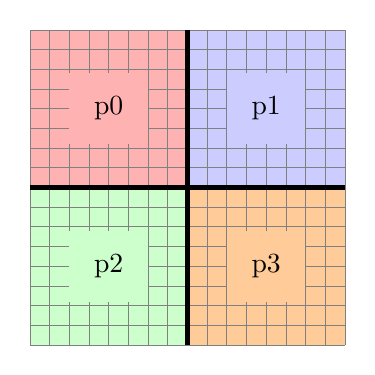
\begin{tikzpicture}
	   \fill [fill=green!20!white] (0,0) -- (2,0) -- (2,2) -- (0,2) -- cycle;
	   \fill [fill=red!30!white]     (0,2) -- (0,4) -- (2,4) -- (2,2) -- cycle;
	   \fill [fill=blue!20!white]    (2,4) -- (4,4) -- (4,2) -- (2,2) -- cycle;
	   \fill [fill=orange!40!white] (4,2) -- (4,0) -- (2,0) -- (2,2) -- cycle;
	   \draw[step=.25cm,gray,very thin] (0,0) grid (4,4);
	   \draw[ultra thick] (0,2) -- (4,2);
	   \draw[ultra thick] (2,4) -- (2,0);
	   \node [fill=red!30!white,draw opacity=1,fill opacity=1,text opacity=1,minimum width=1cm,minimum height=0.9cm] at (1,3) {p0};
	   \node [fill=blue!20!white,draw opacity=1,fill opacity=1,text opacity=1,minimum width=1cm,minimum height=0.9cm] at (3,3) {p1};
	   \node [fill=green!20!white,draw opacity=1,fill opacity=1,text opacity=1,minimum width=1cm,minimum height=0.9cm] at (1,1) {p2};
	   \node [fill=orange!40!white,draw opacity=1,fill opacity=1,text opacity=1,minimum width=1cm,minimum height=0.9cm] at (3,1) {p3};
	\end{tikzpicture}
	\subcaption{Ένα πλέγμα $16*16$, κατανεμημένο σε $4$ διεργασίες, με $64 (8*8)$ στοιχεία η καθεμία.}
	\label{fig:4processes}
\endminipage\hfill
\minipage{0.45\textwidth}
\centering
	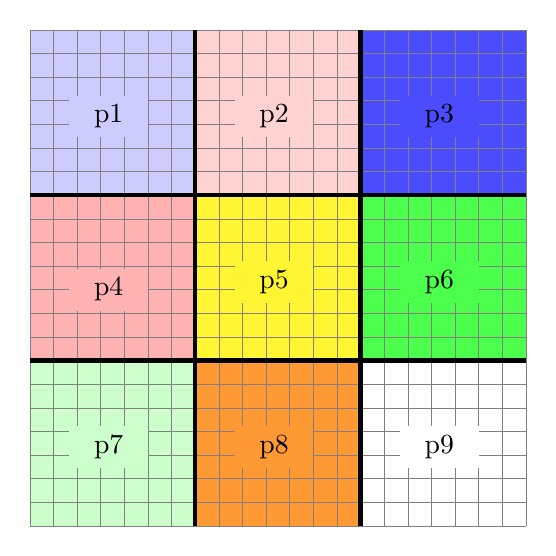
\begin{tikzpicture}
	   \fill [fill=green!20!white]    (0,0) -- (2.1,0) -- (2.1,2.1) -- (0,2.1) -- cycle;
	   \fill [fill=red!30!white]        (0,2.1) -- (0,4.2) -- (2.1,4.2) -- (2.1,2.1) -- cycle;
	   \fill [fill=blue!20!white]      (0,4.2) -- (0,6.3) -- (2.1,6.3) -- (2.1,4.2) -- cycle;
	   \fill [fill=orange!80!white] (2.1,0) -- (2.1,2.1) -- (4.2,2.1) -- (4.2,0) -- cycle;
	   \fill [fill=yellow!80!white]  (2.1,2.1) -- (2.1,4.2) -- (4.2,4.2) -- (4.2,2.1) -- cycle;
	   \fill [fill=pink!70!white]       (2.1,4.2) -- (2.1,6.3) -- (4.2,6.3) -- (4.2,4.2) -- cycle;
	   \fill [fill=blue!70!white]       (4.2,4.2) -- (4.2,6.3) -- (6.3,6.3) -- (6.3,4.2) -- cycle;
	   \fill [fill=green!70!white]    (4.2,2.1) -- (4.2,4.2) -- (6.3,4.2) -- (6.3,2.1) -- cycle;
	   \draw[step=.3cm,gray,very thin] (0,0) grid (6.3,6.3);
	   \draw[ultra thick] (0,2.1) -- (6.3,2.1);
	   \draw[ultra thick] (0,4.2) -- (6.3,4.2);
	   \draw[ultra thick] (2.1,0) -- (2.1,6.3);
	   \draw[ultra thick] (4.2,0) -- (4.2,6.3);
	   \node [fill=green!20!white,draw opacity=1,fill opacity=1,text opacity=1,minimum width=1cm,minimum height=0.4cm] at (1,1) {p7};
	   \node [fill=red!30!white,draw opacity=1,fill opacity=1,text opacity=1,minimum width=1cm,minimum height=0.4cm] at (1,3) {p4};
	   \node [fill=blue!20!white,draw opacity=1,fill opacity=1,text opacity=1,minimum width=1cm,minimum height=0.4cm] at (1,5.2) {p1};
	   \node [fill=orange!80!white,draw opacity=1,fill opacity=1,text opacity=1,minimum width=1cm,minimum height=0.4cm] at (3.1,1) {p8};
	   \node [fill=yellow!80!white,draw opacity=1,fill opacity=1,text opacity=1,minimum width=1cm,minimum height=0.4cm] at (3.1,3.1) {p5};
	   \node [fill=pink!70!white,draw opacity=1,fill opacity=1,text opacity=1,minimum width=1cm,minimum height=0.4cm] at (3.1,5.2) {p2};
	   \node [fill=white,draw opacity=1,fill opacity=1,text opacity=1,minimum width=1cm,minimum height=0.4cm] at (5.2,1) {p9};
	   \node [fill=green!70!white,draw opacity=1,fill opacity=1,text opacity=1,minimum width=1cm,minimum height=0.4cm] at (5.2,3.1) {p6};
	   \node [fill=blue!70!white,draw opacity=1,fill opacity=1,text opacity=1,minimum width=1cm,minimum height=0.4cm] at (5.2,5.2) {p3};
	\end{tikzpicture}
	\subcaption{Ένα πλέγμα $21*21$, κατανεμημένο σε $9$ διεργασίες, με $49 (7*7)$ στοιχεία η καθεμία.}
	\label{fig:9processes}
\endminipage

	\caption{Διάφορες πιθανές καρτεσιανές τοπολογίες. Δεν περιλαμβάνονται οι άλω της κάθε διεργασίας στα σχήματα.}
	\label{fig:cartesian}
\end{figure}

\begin{figure}[h]
\centering
\minipage{.4\textwidth}
\centering
	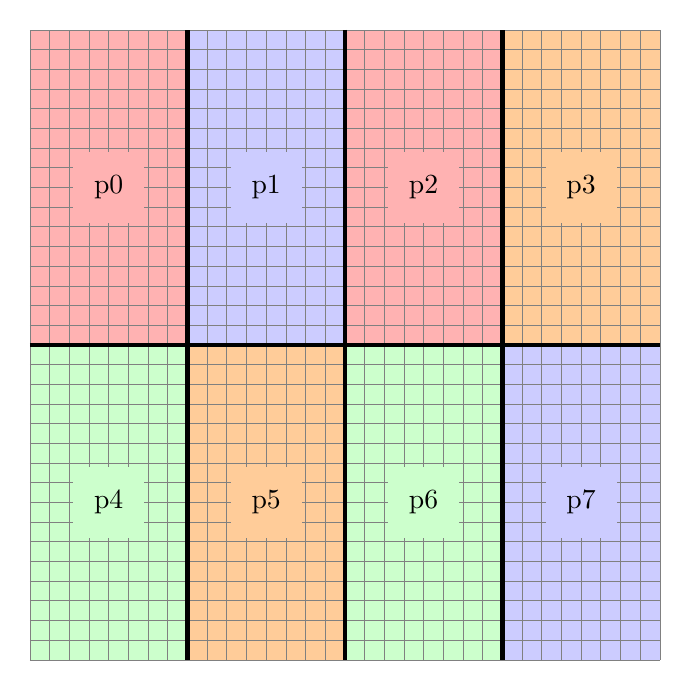
\begin{tikzpicture}
	   \fill [fill=green!20!white] (0,0) -- (2,0) -- (2,4) -- (0,4) -- cycle;
	   \fill [fill=red!30!white]     (0,4) -- (0,8) -- (2,8) -- (2,4) -- cycle;
	   \fill [fill=blue!20!white]    (2,8) -- (4,8) -- (4,4) -- (2,4) -- cycle;
	   \fill [fill=orange!40!white] (4,4) -- (4,0) -- (2,0) -- (2,4) -- cycle;
	   \fill [fill=green!20!white] (4,0) -- (4,4) -- (6,4) -- (6,0) -- cycle;
	   \fill [fill=red!30!white]     (4,4) -- (4,8) -- (6,8) -- (6,4) -- cycle;
	   \fill [fill=blue!20!white]    (6,0) -- (6,4) -- (8,4) -- (8,0) -- cycle;
	   \fill [fill=orange!40!white] (6,4) -- (6,8) -- (8,8) -- (8,4) -- cycle;
	   \draw[step=.25cm,gray,very thin] (0,0) grid (8,8);
	   \draw[ultra thick] (0,4) -- (8,4);
	   \draw[ultra thick] (2,0) -- (2,8);
	   \draw[ultra thick] (6,0) -- (6,8);
	   \draw[ultra thick] (4,8) -- (4,0);
	   \node [fill=red!30!white,draw opacity=1,fill opacity=1,text opacity=1,minimum width=.9cm,minimum height=.9cm] at (1,6) {p0};
	   \node [fill=blue!20!white,draw opacity=1,fill opacity=1,text opacity=1,minimum width=.9cm,minimum height=.9cm] at (3,6) {p1};
	   \node [fill=green!20!white,draw opacity=1,fill opacity=1,text opacity=1,minimum width=.9cm,minimum height=.9cm] at (1,2) {p4};
	   \node [fill=orange!40!white,draw opacity=1,fill opacity=1,text opacity=1,minimum width=.9cm,minimum height=.9cm] at (3,2) {p5};
	   \node [fill=red!30!white,draw opacity=1,fill opacity=1,text opacity=1,minimum width=.9cm,minimum height=.9cm] at (5,6) {p2};
	   \node [fill=blue!20!white,draw opacity=1,fill opacity=1,text opacity=1,minimum width=.9cm,minimum height=.9cm] at (7,2) {p7};
	   \node [fill=green!20!white,draw opacity=1,fill opacity=1,text opacity=1,minimum width=.9cm,minimum height=.9cm] at (5,2) {p6};
	   \node [fill=orange!40!white,draw opacity=1,fill opacity=1,text opacity=1,minimum width=.9cm,minimum height=.9cm] at (7,6) {p3};
	\end{tikzpicture}
	\subcaption{$4*2$}
	\label{fig:4processes}
\endminipage\\
\minipage{.4\textwidth}
\centering
	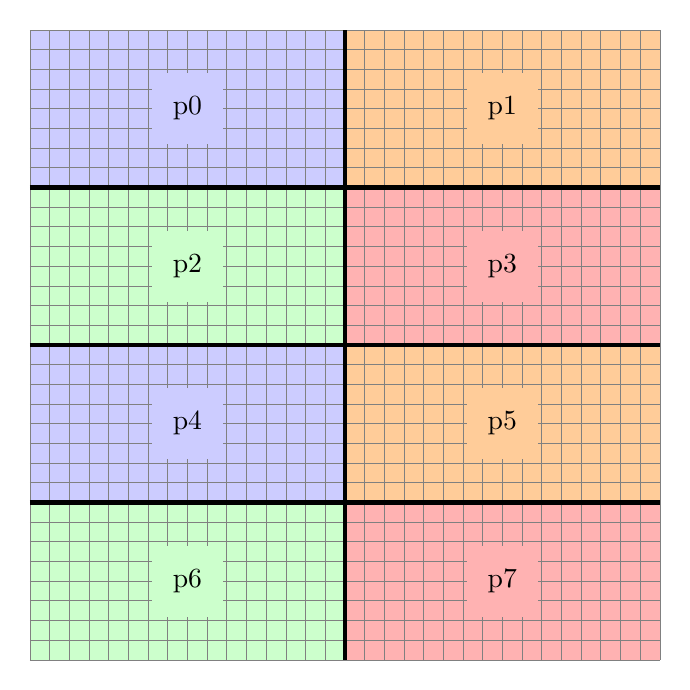
\begin{tikzpicture}
	   \fill [fill=green!20!white] (0,0) -- (4,0) -- (4,2) -- (0,2) -- cycle;
	   \fill [fill=red!30!white]     (4,0) -- (8,0) -- (8,2) -- (4,2) -- cycle;
	   \fill [fill=blue!20!white]    (0,2) -- (4,2) -- (4,4) -- (0,4) -- cycle;
	   \fill [fill=orange!40!white] (4,2) -- (8,2) -- (8,4) -- (4,4) -- cycle;
	   \fill [fill=green!20!white] (0,4) -- (4,4) -- (4,6) -- (0,6) -- cycle;
	   \fill [fill=red!30!white]     (4,4) -- (8,4) -- (8,6) -- (4,6) -- cycle;
	   \fill [fill=blue!20!white]    (0,6) -- (4,6) -- (4,8) -- (0,8) -- cycle;
	   \fill [fill=orange!40!white] (4,6) -- (8,6) -- (8,8) -- (4,8) -- cycle;
	   \draw[step=.25cm,gray,very thin] (0,0) grid (8,8);
	   \draw[ultra thick] (0,2) -- (8,2);
	   \draw[ultra thick] (0,4) -- (8,4);
	   \draw[ultra thick] (0,6) -- (8,6);
	   \draw[ultra thick] (4,0) -- (4,8);
	   \node [fill=red!30!white,draw opacity=1,fill opacity=1,text opacity=1,minimum width=.9cm,minimum height=.9cm] at (6,1) {p7};
	   \node [fill=blue!20!white,draw opacity=1,fill opacity=1,text opacity=1,minimum width=.9cm,minimum height=.9cm] at (2,3) {p4};
	   \node [fill=green!20!white,draw opacity=1,fill opacity=1,text opacity=1,minimum width=.9cm,minimum height=.9cm] at (2,1) {p6};
	   \node [fill=orange!40!white,draw opacity=1,fill opacity=1,text opacity=1,minimum width=.9cm,minimum height=.9cm] at (6,3) {p5};
	   \node [fill=red!30!white,draw opacity=1,fill opacity=1,text opacity=1,minimum width=.9cm,minimum height=.9cm] at (6,5) {p3};
	   \node [fill=blue!20!white,draw opacity=1,fill opacity=1,text opacity=1,minimum width=.9cm,minimum height=.9cm] at (2,7) {p0};
	   \node [fill=green!20!white,draw opacity=1,fill opacity=1,text opacity=1,minimum width=.9cm,minimum height=.9cm] at (2,5) {p2};
	   \node [fill=orange!40!white,draw opacity=1,fill opacity=1,text opacity=1,minimum width=.9cm,minimum height=.9cm] at (6,7) {p1};
	\end{tikzpicture}
	\subcaption{$2*4$}
\endminipage
	\caption{Ένα πλέγμα $32*32$, κατανεμημένο με δύο διαφορετικούς τρόπους σε $8$ διεργασίες, με $128 (16*8)$ στοιχεία η καθεμία.}
	\label{fig:8processes}
\end{figure}

\clearpage
Αφού τρέξουμε το δοκιμαστικό πρόγραμμα, παίρνουμε το παρακάτω output από το MPI\footnote{Το αρχείο μπορεί να βρεθεί στο directory \path{/home/pool/argo029/GameOfLife/MPI/Results/Verification}}

\begin{figure}[h]
\begin{tcolorbox}
mpiP: \\
mpiP: mpiP: mpiP V3.4.1 (Build Oct 27 2018/17:18:21) \\
mpiP: Direct questions and errors to mpip-help@lists.sourceforge.net \\
mpiP:  \\
rows are 10 \\
columns are 10 \\
\\
The cartesian topology for process 0 is \\
0, 0 \\
north 2 \\
east 1 \\
west 1 \\
south 2 \\
northwest 3 \\
northeast 3 \\
southeast 3 \\
southwest 3 \\
\end{tcolorbox}
\caption{Το output της διεργασίας $0$ μας περιγράφει την καρτεσιανή τοπολογία, καθώς και τον αριθμό σειρών και στηλών}
\label{fig:verification}
\end{figure}

\begin{multicols}{2}
Όπως είδαμε και στον κώδικα, το output γράφεται αποκλειστικά από την διεργασία $0$. Παρατηρούμε πως η τοπολογία συμμορφώνεται με το Σχήμα \ref{fig:4processes}. Αρχικά βλέπουμε πως η διεργασία έχει $10$ σειρές και $10$ στήλες, το οποίο είναι και σωστό, αφού στην κάθε διεργασία αντιστοιχούν $8$ σειρές και στήλες, συν άλλες $2$ σε κάθε διάσταση για να συμπεριληφθούν οι άλω. \par
Στη συνέχεια βλέπουμε πως οι συντεταγμένες της διεργασίας είναι οι $(0,0)$. Μετά ακολουθούν δηλώσεις για το ποιοι είναι οι γείτονες της διεργασίας, πχ βλέπουμε πως νοτιοδυτικά βρίσκεται η διεργασία $3$. Μία γρήγορη ματιά στο σχήμα \ref{fig:4processes} επιβεβαιώνει πως και οι γείτονες της διεργασίας εντοπίζονται σωστά από το πρόγραμμα. \par
Ακολουθεί το output του πλέγματος μετά την αρχικοποίηση με τυχαίες τιμές, και \emph{πριν} το κύριο loop.
\begin{tcolorbox}
\centering
The grid for process 0 is: \\
0 0 0 0 0 0 0 0 0 0 \\
0 1 1 0 0 0 0 1 0 0 \\
0 1 1 1 0 0 0 1 0 0 \\
0 0 1 1 0 1 1 1 0 0 \\
0 0 1 1 0 0 0 1 1 0 \\
0 1 1 1 0 0 1 0 1 0 \\
0 0 0 0 1 0 1 1 1 0 \\
0 1 1 1 1 0 1 1 1 0 \\
0 1 1 0 1 1 1 1 1 0 \\
0 0 0 0 0 0 0 0 0 0 \\
\end{tcolorbox}

Παρατηρούμε πως όλα τα στοιχεία των άλω έχουν την τιμή $0$, καθώς δεν έχει ξεκινήσει ακόμα η ανταλλαγή στοιχείων. Με μία ματιά στο αρχείο εξόδου μπορούμε να δούμε και τα πλέγματα των υπόλοιπων διεργασιών (παραλείπονται από το κείμενο για λόγους αναγνωσιμότητας). \par
Ξεκινά το παιχνίδι, το οποίο και θα κρατήσει $5$ γενεές. Σε κάθε γενιά, τυπώνεται ο αριθμός της, και στη συνέχεια το πλέγμα της κάθε διεργασίας. Για την διεργασία $0$, έχουμε:

\begin{tcolorbox}
Generation 0: \\
The grid for process 0 is: \\
1 1 0 1 1 1 1 0 1 1 \\
1 1 1 0 0 0 0 1 0 1 \\
1 1 1 1 0 0 0 1 0 1 \\
1 0 1 1 0 1 1 1 0 0 \\
1 0 1 1 0 0 0 1 1 0 \\
0 1 1 1 0 0 1 0 1 0 \\
1 0 0 0 1 0 1 1 1 0 \\
1 1 1 1 1 0 1 1 1 1 \\
0 1 1 0 1 1 1 1 1 0 \\
0 1 0 0 0 0 0 0 1 0 \\
\end{tcolorbox}

Δεν έχει ξεκινήσει ακόμη ο υπολογισμός της επόμενης γενιάς, τώρα το μόνο που συνέβη ήταν η ανταλλαγή των άλω. Πρέπει να επαληθεύσουμε πως η ανταλλαγή έγινε σωστά. \par

\textbf{Η βόρεια άλω} περιέχει τα στοιχεία \\ \emph{1 0 1 1 1 1 0 1} (σαφώς και δεν περιλαμβάνονται τα γωνιακά στοιχεία). Πρέπει να ελέγξουμε τα στοιχεία στην τελευταία σειρά της διεργασίας που βρίσκεται βόρεια, δηλαδή της $2$. Στο αρχείο εξόδου βλέπουμε τα παρακάτω. Επιλέχθηκε το output χωρίς τις άλω, προτού ξεκινήσει το παιχνίδι, για να είναι πιο ευδιάκριτα τα στοιχεία. 
\begin{tcolorbox}
The grid for process 2 is: \\
0 0 0 0 0 0 0 0 0 0 \\
0 1 0 0 0 0 0 0 1 0 \\
0 0 0 1 0 1 1 1 0 0 \\
0 1 0 1 0 0 0 1 1 0 \\
0 0 0 0 1 0 1 1 0 0 \\
0 1 0 0 0 0 1 1 1 0 \\
0 0 0 1 1 1 1 0 1 0 \\
0 1 1 1 1 1 0 1 0 0 \\
0 1 0 1 1 1 1 0 1 0 \\
0 0 0 0 0 0 0 0 0 0 \\
\end{tcolorbox}
Βλέπουμε πως πράγματι η τελευταία σειρά της διεργασίας είναι ίδια με την βόρεια άλω. \par
\textbf{Η νότια άλω} περιέχει τα στοιχεία \\ \emph{1 0 0 0 0 0 0 1} και προέρχεται επίσης από την διεργασία $2$. Η πρώτη σειρά της διεργασίας $2$ είναι ίδια με την άλω μας, οπότε επαληθεύεται και εδώ η σωστή ανταλλαγή. \par
\textbf{Η ανατολική άλω} περιέχει τα στοιχεία \emph{1 1 0 0 0 0 1 0}. Η διεργασία που βρίσκεται ανατολικά είναι η $1$, το πλέγμα της οποίας έχει ως εξής:

\begin{tcolorbox}
The grid for process 1 is: \\
0 0 0 0 0 0 0 0 0 0 \\
0 1 0 0 0 0 0 1 1 0 \\
0 1 0 0 0 0 1 1 1 0 \\
0 0 0 0 0 0 0 0 1 0 \\
0 0 1 1 1 0 1 1 1 0 \\
0 0 0 0 0 0 1 0 0 0 \\
0 0 0 1 0 1 1 0 1 0 \\
0 1 0 0 0 0 0 1 1 0 \\
0 0 0 0 0 0 1 0 0 0 \\
0 0 0 0 0 0 0 0 0 0 \\
\end{tcolorbox}

Η αριστερότερη στήλη έχει τις ίδιες τιμές με την άλω, οπότε επαληθεύονται ξανά τα αποτελέσματα. \par

\textbf{Η δυτική άλω} έχει τα στοιχεία \\ \emph{1 1 1 1 0 1 1 0}. Η άλω αυτή προέρχεται επίσης από την $1$, της οποίας η δεξιότερη στήλη έχει τις ίδιες τιμές. \par
\textbf{Τα γωνιακά στοιχεία} προέρχονται όλα από την διεργασία $3$, το πλέγμα της οποίας είναι:

\begin{tcolorbox}
The grid for process 3 is: \\
0 0 0 0 0 0 0 0 0 0 \\
0 0 0 1 0 0 0 0 0 0 \\
0 0 1 0 0 1 0 0 0 0 \\
0 0 0 0 0 0 0 0 0 0 \\
0 0 1 1 0 0 1 0 1 0 \\
0 0 0 1 0 1 0 1 0 0 \\
0 1 1 0 1 1 1 0 0 0 \\
0 0 1 0 0 0 1 1 0 0 \\
0 1 1 0 0 1 1 1 1 0 \\
0 0 0 0 0 0 0 0 0 0 \\
\end{tcolorbox}
Παρατηρώντας τα τέσσερα γωνιακά στοιχεία και συγκρίνοντάς τα με τα άλω, βλέπουμε πως είναι και εδώ σωστές οι τιμές. \par
Με βάση τα παραπάνω, οδηγούμαστε στο συμπέρασμα πως η ανταλλαγή όλων των στοιχείων λειτουργεί σωστά. Μένει μόνο να επαληθεύσουμε πως και ο υπολογισμός της κάθε γενιάς γίνεται σωστά. \par
Παραθέτουμε για την διεργασία $0$ τις γενιές $0$ και $1$.

\begin{tcolorbox}[left=2pt,right=2pt]
\centering
\textbf{Generation 0} \quad \textbf{Generation 1} \\
1 1 0 1 1 1 1 0 1 1 \quad 0 0 0 0 0 0 0 0 0 0 \\
1 1 1 0 0 0 0 1 0 1 \quad 0 0 0 0 0 1 0 1 0 0 \\
1 1 1 1 0 0 0 1 0 1 \quad 0 0 0 0 1 0 0 1 0 0 \\
1 0 1 1 0 1 1 1 0 0 \quad 0 0 0 0 0 0 0 0 0 1 \\
1 0 1 1 0 0 0 1 1 0 \quad 1 0 0 0 0 1 0 0 1 1 \\
0 1 1 1 0 0 1 0 1 0 \quad 0 0 0 0 1 1 1 0 0 0 \\
1 0 0 0 1 0 1 1 1 0 \quad 0 0 0 0 1 0 0 0 0 0 \\
1 1 1 1 1 0 1 1 1 1 \quad 0 0 0 0 0 0 0 0 0 1 \\
0 1 1 0 1 1 1 1 1 0 \quad 0 0 0 0 1 0 0 0 0 0 \\
0 1 0 0 0 0 0 0 1 0 \quad 0 1 0 1 0 0 0 0 1 1 \\
\end{tcolorbox}

Ελέγχοντας τα παραπάνω πλέγματα, είναι εύκολο να δούμε πως ο υπολογισμός της επόμενης γενιάς πραγματοποιείται σωστά. Είμαστε λοιπόν έτοιμοι να ξεκινήσουμε με τις μετρήσεις, αφού φυσικά απενεργοποιήσουμε τα macros που χρησιμεύουν στο debugging. Το ακολουθιακό πρόγραμμα με μία μόνο MPI διεργασία, έχει χρόνο εκτέλεσης 11.5\si{\second} για $2000$ γενιές και μέγεθος πλέγαμτος $840$. Θα επιλεχθούν αυτές οι τιμές ως αφετηρία.
\end{multicols}

%%%%%%%%%%%%%%%%%%%%%%%%%%%%%%%%%%%%%%%%%%%%%%%%%%%%%%%%%%%%%%%%%%%%%
\section{Μετρήσεις στην Αργώ με μεθοδολογία block -- block}

Ακολουθούν οι πίνακες των χρόνων, επιτάχυνσης και αποδοτικότητας από τις μετρήσεις στην Αργώ. Στον πίνακα των χρόνων, ο οποίος απεικονίζεται \emph{σε δευτερόλεπτα}, με την τιμή «Ε» συμπληρώνονται τα κελιά για τα οποία δεν έχουν νόημα οι μετρήσεις, εφόσον εντοπίστηκε επιβράδυνση.

\begin{table}[h]
\centering
\begin{tabular}{|l| c | c | c | c | c | c | c | c | c |}
\hline
\diagbox{Μέγεθος}{Διεργασίες} & 1 & 4 & 9 & 16 & 25 & 36 & 49 & 64 & 80\\
\hline
840 & 11.5 & 2.94 & 0.91 & 0.62 & 0.59 & 0.56 & 0.58 & Ε & Ε \\
\hline
1680 & 46.12 & 11.59 & 5.38 & 3.10 & 1.28 & 0.99 & 0.84 & 0.77 & 0.72 \\
\hline
3360 & 185.29 & 46.24 & 20.86 & 11.77 & 7.7 & 5.49 & 4.11 & 3.24 & 2.72 \\
\hline
6720 & 740.34 & 186.46 & 84.08 & 47.78 & 30.51 & 20.99 & 15.47 & 11.91 & 9.62 \\
\hline
13440 & 2959 & 743.77 & 332.44 & 188.54 & 121.2 & 84.73 & 62.43 & 48.12 & 38.53 \\
\hline
26880 &&&&&&&&& \\
\hline
\end{tabular}
\caption{Χρόνοι για καθαρά MPI}
\label{tab:timesMPI}
\end{table}

\begin{table}[h]
\centering
\begin{tabular}{|l| c | c | c | c | c | c | c | c | c |}
\hline
\diagbox{Μέγεθος}{Διεργασίες} & 1 & 4 & 9 & 16 & 25 & 36 & 49 & 64 & 80\\
\hline
840 & 1 & 3.9 & 12.6 & 18.5 & 19.4 & 20.5 & 19.8 & Ε & Ε \\
\hline
1680 & 1 & 3.9 & 8.5 & 14.8 & 36 & 46.5 & 54.9 & 59.8 & 64 \\
\hline
3360 & 1 & 4 & 8.8 & 15.7 & 24 & 33.7 & 45 & 57.1 & 68.1 \\
\hline
6720 & 1 & 3.9 & 8.8 & 15.4 & 24.2 & 35.2 & 47.8 & 62.1 & 76.9 \\
\hline
13440 & 1 & 3.9 & 8.9 & 15.6 & 24.4 & 34.9 & 47.3 & 61.4 & 76.7 \\
\hline
26880 & 1 &&&&&&&& \\
\hline
\end{tabular}
\caption{Επιτάχυνση ($S = Ts / Tp$) για καθαρά MPI}
\label{tab:speedupMPI}
\end{table}

\begin{table}[h]
\centering
\begin{tabular}{|l| c | c | c | c | c | c | c | c | c |}
\hline
\diagbox{Μέγεθος}{Διεργασίες} & 1 & 4 & 9 & 16 & 25 & 36 & 49 & 64 & 80\\
\hline
840 & 1 & 0.97 & 1.4 & 1.15 & 0.77 & 0.56 & 0.4 & N/A & N/A \\
\hline
1680 & 1 & 0.97 & 0.94 & 0.92 & 1.44 & 1.29 & 1.12 & 0.93 & 0.8 \\
\hline
3360 & 1 & 1 & 0.97 & 0.98 & 0.96 & 0.93 & 0.91 & 0.89 & 0.85 \\
\hline
6720 & 1 & 0.97 & 0.94 & 0.96 & 0.96 & 0.97 & 0.97 & 0.97 & 0.96 \\
\hline
13440 & 1 & 0.97 & 0.38 & 0.97 & 0.97 & 0.96 & 0.96 & 0.95 & 0.95 \\
\hline
26880 & 1 &&&&&&&& \\
\hline
\end{tabular}
\caption{Αποδοτικότητα ($E = S / p$) για καθαρά MPI}
\label{tab:efficiencyMPI}
\end{table}

%%%%%%%%%%%%%%%%%%%%%%%%%%%%%%%%%%%%%%%%%%%%%%%%%%%%%%%%%%%%%%%%%%%%%
\section{Μετρήσεις στην Αργώ με μεθοδολογία σειρών}
Ακολουθούν οι πίνακες των χρόνων, επιτάχυνσης και αποδοτικότητας από τις μετρήσεις στην Αργώ. Στον πίνακα των χρόνων, με την τιμή «Ε» συμπληρώνονται τα κελιά για τα οποία δεν έχουν νόημα οι μετρήσεις, εφόσον εντοπίστηκε επιβράδυνση.

\begin{table}[h]
\centering
\begin{tabular}{|l| c | c | c | c | c | c | c | c | c |}
\hline
\diagbox{Μέγεθος}{Διεργασίες} & 1 & 4 & 9 & 16 & 25 & 36 & 49 & 64 & 80\\
\hline
840 & 11.5 & 2.94 & 0.91 & 0.62 & 0.59 & 0.56 & 0.58 & Ε & Ε \\
\hline
1680 & 46.12 & 11.59 & 5.38 & 3.10 & 1.28 & 0.99 & 0.84 & 0.77 & 0.72 \\
\hline
3360 & 185.29 & 46.24 & 20.86 & 11.77 & 7.7 & 5.49 & 4.11 & 3.24 & 2.72 \\
\hline
6720 & 740.34 & 186.46 & 84.08 & 47.78 & 30.51 & 20.99 & 15.47 & 11.91 & 9.62 \\
\hline
13440 & \\
\hline
\end{tabular}
\caption{Χρόνοι για καθαρά MPI}
\label{tab:timesMPIrows}
\end{table}

\begin{table}[h]
\centering
\begin{tabular}{|l| c | c | c | c | c | c | c | c | c |}
\hline
\diagbox{Μέγεθος}{Διεργασίες} & 1 & 4 & 9 & 16 & 25 & 36 & 49 & 64 & 80\\
\hline
840 & 1 & 3.9 & 12.6 & 18.5 & 19.4 & 20.5 & 19.8 & Ε & Ε \\
\hline
1680 & 1 & 3.9 & 8.5 & 14.8 & 36 & 46.5 & 54.9 & 59.8 & 64 \\
\hline
3360 & 1 & 4 & 8.8 & 15.7 & 24 & 33.7 & 45 & 57.1 & 68.1 \\
\hline
6720 & 1 & 3.9 & 8.8 & 15.4 & 24.2 & 35.2 & 47.8 & 62.1 & 76.9 \\
\hline
13440 & \\
\hline
\end{tabular}
\caption{Επιτάχυνση ($S = Ts / Tp$) για καθαρά MPI}
\label{tab:speedupMPIrows}
\end{table}

\begin{table}[h]
\centering
\begin{tabular}{|l| c | c | c | c | c | c | c | c | c |}
\hline
\diagbox{Μέγεθος}{Διεργασίες} & 1 & 4 & 9 & 16 & 25 & 36 & 49 & 64 & 80\\
\hline
840 & 1 & 0.975 & 1.4 & 1.15 & 0.77 & 0.56 & 0.4 & N/A & N/A \\
\hline
1680 & 1 & 0.975 & 0.94 & 0.92 & 1.44 & 1.29 & 1.12 & 0.93 & 0.8 \\
\hline
3360 & 1 & 1 & 0.97 & 0.98 & 0.96 & 0.93 & 0.91 & 0.89 & 0.85 \\
\hline
6720 & 1 & 0.97 & 0.94 & 0.96 & 0.96 & 0.97 & 0.97 & 0.97 \\
\hline
13440 & 1 & \\
\hline
\end{tabular}
\caption{Αποδοτικότητα ($E = S / p$) για καθαρά MPI}
\label{tab:efficiencyMPIrows}
\end{table}

%%%%%%%%%%%%%%%%%%%%%%%%%%%%%%%%%%%%%%%%%%%%%%%%%%%%%%%%%%%%%%%%%%%%%
\section{Παρατηρήσεις και συμπεράσματα}